\documentclass[a4paper, 11pt]{article} % Font size (can be 10pt, 11pt or 12pt) and paper size (remove a4paper for US letter paper)
\usepackage{helvet}
\renewcommand{\familydefault}{\sfdefault}
\usepackage[protrusion=true,expansion=true]{microtype} % Better typography
\usepackage{graphicx} % Required for including pictures
\usepackage[usenames,dvipsnames]{color} % Coloring code
\usepackage{wrapfig} % Allows in-line images
\usepackage[utf8]{inputenc}
\usepackage{enumerate}
\usepackage{enumitem}
\usepackage{framed, color}
\definecolor{shadecolor}{rgb}{0.690, 0.933, 0.525}

% Imágenes
\usepackage{graphicx} 

\usepackage{amsmath}
% para importar svg
%\usepackage[generate=all]{svgfig}

% sudo apt-get install texlive-lang-spanish
\usepackage[spanish]{babel} % English language/hyphenation
\selectlanguage{spanish}
% Hay que pelearse con babel-spanish para el alineamiento del punto decimal
\decimalpoint
\usepackage{dcolumn}
\newcolumntype{d}[1]{D{.}{\esperiod}{#1}}
\makeatletter
\addto\shorthandsspanish{\let\esperiod\es@period@code}
\makeatother

\usepackage{longtable}
\usepackage{tabu}
\usepackage{supertabular}

\usepackage{multicol}
\newsavebox\ltmcbox

% Para algoritmos
\usepackage{algorithm}
\usepackage{algorithmic}
\usepackage{amsthm}

% Para matrices
\usepackage{amsmath}

% Símbolos matemáticos
\usepackage{amssymb}
\usepackage{accents}
\let\oldemptyset\emptyset
\let\emptyset\varnothing

\usepackage[hidelinks]{hyperref}

\usepackage[section]{placeins} % Para gráficas en su sección.
\usepackage[T1]{fontenc} % Required for accented characters
\usepackage{tikz}
\newenvironment{allintypewriter}{\ttfamily}{\par}
\setlength{\parindent}{0pt}
\parskip=8pt
\linespread{1.05} % Change line spacing here, Palatino benefits from a slight increase by default

\makeatletter
\renewcommand\@biblabel[1]{\textbf{#1.}} % Change the square brackets for each bibliography item from '[1]' to '1.'
\renewcommand{\@listI}{\itemsep=0pt} % Reduce the space between items in the itemize and enumerate environments and the bibliography
\newcommand{\imagen}[2]{\begin{center} \includegraphics[width=90mm]{#1} \\#2 \end{center}}
\newcommand{\RFC}[1]{\href{https://www.ietf.org/rfc/rfc#1.txt}{RFC-#1}}

\renewcommand{\maketitle}{ % Customize the title - do not edit title and author name here, see the TITLE block below
\begin{center} % Center align
{\Huge\@title} % Increase the font size of the title
\end{center}

\vspace{20pt} % Some vertical space between the title and author name

\begin{flushright} % Right align
{\large\@author} % Author name
\\\@date % Date

\vspace{40pt} % Some vertical space between the author block and abstract
\end{flushright}
\renewcommand{\baselinestretch}{0.5}

}


\usepackage[a4paper]{geometry}
\geometry{top=2cm, bottom=2cm, left=2.25cm, right=2.25cm}

%----------------------------------------------------------------------------------------
%	TITLE
%----------------------------------------------------------------------------------------

\title{\textbf{Computación, Machine Learning}\\ % Title
\vspace{20 pt}
Historia de las Matemáticas} % Subtitle

\author{\textsc{Daniel López García\\
Lothar Soto Palma\\
Elena Toro Pérez} % Author
\\{\textit{Universidad de Granada}}} % Institution

\date{\today} % Date

\newcounter{ndef}

\begin{document}
	\maketitle
	\tableofcontents
	\listoffigures

\section{Introduccion}
		Lista de temas a tratar:
		\begin{itemize}
			\item Antecedentes estadísticos
			\item Máquina de aprendizaje de Turing
			\item Neural Network
			\item Perceptron
			\item Máquinas y juegos
			\item Nearest Neighbor
			\item Stanford cart y otros experimentos
			\item Neocognitron
			\item Backpropagation
			\item Algoritmos de aprendizaje
			\item Final con el estado actual del machine learning
		\end{itemize}
				
\section{Historia General}

\newpage

\section{Temas 1 por 1}
\subsection{Introducción}
\textbf{Machine learning} es una disciplina científica del ámbito de la Inteligencia Artificial que crea sistemas que aprenden automáticamente.

Pero, ¿qué significan las palabras aprender y automáticamente, en este contexto?

\textit{Aprender} en este contexto quiere decir identificar patrones complejos en millones de datos. La máquina que realmente aprende es un algoritmo que revisa los datos y es capaz de predecir comportamientos futuros. 

\textit{Automáticamente}, también en este contexto, implica que estos sistemas se mejoran de forma autónoma con el tiempo, sin intervención humana.

Hoy en día, podemos observar la aplicación concreta de Machine Learning en varios campos que nos rodean, como son:
		\begin{itemize}
		    \item \textbf{Automóviles:} Sistemas de piloto automático, Detección de fallos por reconocimiento externo de vibraciones...
		    \item \textbf{Bancos:} Lectura de cheques y otros documentos, Detección de fraude en transacciones...
		    \item \textbf{Electrónica:} Reconocimiento de voz, visión artificial...
		    \item \textbf{Finanzas:} Asesoría de préstamos (aceptación/denegación de un crédito), Identificación de falsificaciones, Interpretación y reconocimiento de firmas...
		    \item \textbf{Internet:} Compras on-line, Anuncios on-line, Selección de clientes potenciales basándose en comportamientos en las redes sociales, interacciones en la web...
		    \item \textbf{Manufactura:}  Inspección de calidad mediante sistemas visuales, Control de la producción y del proceso, Análisis y diseño de productos....
		    \item \textbf{Medicina:} Análisis de células portadoras de cáncer mamario, Diseño de prótesis, Diseño de prediagnósticos médicos basados en síntomas del paciente...
		    \item \textbf{Recursos Humanos:} Predicción de qué empleados serán más rentables el año que viene.
		    \item \textbf{Robótica:} Control dinámico de trayectoria, Sistemas ópticos...
		    \item \textbf{Seguridad:} Reconocimiento de huellas digitales, Criptografía...		\item \textbf{Telecomunicaciones:} Compresión de datos e imágenes, Automatización de servicios de información, Decidir cuál es la mejor hora para llamar a un cliente...
		    \item \textbf{Transporte:} Sistemas de rutas y seguimiento de flotas, Diagnóstico de frenos en camiones...
		    \item \textbf{Voz:} Reconocimiento de voz, Transformación de texto escrito a voz...
		\end{itemize}
		
\underline{Un ejemplo concreto} de aplicación de esta técnica puede ser el siguiente:

\begin{shaded}
Una empresa de telefonía quiere saber qué clientes están en “peligro” de darse de baja de sus servicios para hacer acciones comerciales que eviten que se vayan a la competencia.

¿Cómo puede hacerlo? La empresa tiene muchos datos de los clientes, pero seguramente los usa solo para facturar y para hacer estadísticas.

¿Qué más puede hacer con esos datos? Se pueden usar para predecir cuándo un cliente se va a dar de baja y gestionar la mejor acción que lo evite.

Los datos históricos del conjunto de los clientes, debidamente organizados y tratados en bloque, generan una base de datos que se puede explotar para predecir futuros comportamientos (favorecer aquellos que mejoran los objetivos de negocio y evitar aquellos que son perjudiciales).

Esa cantidad inmensa de datos son imposibles de analizar por una persona para sacar conclusiones y menos todavía para hacer predicciones. Los algoritmos en cambio sí pueden detectar patrones de comportamiento contando con las variables que le proporcionamos y descubrir cuáles son las que han llevado, en este caso, a darse de baja como cliente.
\end{shaded}

\begin{figure}[H]
\centering
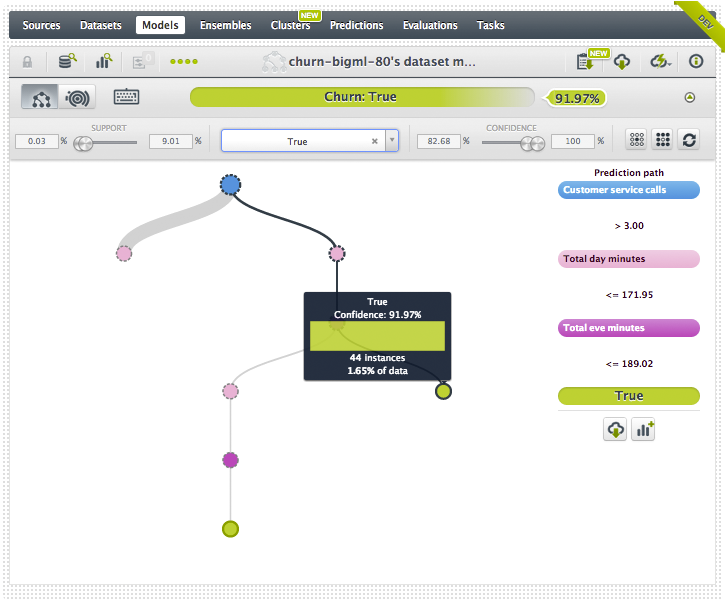
\includegraphics[width=0.95\textwidth]{ejemploMachineLearning.png}
\caption{Ejemplo de una predicción simplificada basada en datos de una compañía de telefonía ficticia, pero usando una herramienta de Machine Learning real}
\label{Ejemplo de una predicción simplificada basada en datos de una compañía de telefonía ficticia, pero usando una herramienta de Machine Learning real}
\end{figure}


\begin{shaded}
La visualización en árbol (en esta imagen está simplificado) permite ver los patrones que han seguido ciertos clientes que se han dado de baja.

En este caso está resaltada una de las ramas centrales, que indican un patrón en el que el cliente:
\begin{itemize}
    \item Tiene más de $3$ llamadas al servicio de atención al cliente.
    \item Llama menos de $171,95$ minutos al día.
    \item Las llamadas en horario nocturno son inferiores a $189,02$ minutos.
\end{itemize}

Por tanto, la predicción sería: \textit{Si los clientes que tienen estas características ya se han dado de baja de la compañía, es previsible que los que todavía son clientes y tienen este mismo comportamiento estén en riesgo de irse. Según este modelo predictivo, es bastante probable que esto suceda (se dice que la predicción tiene una confianza, en este caso, del $91,97\%$).}

Si el departamento de marketing tuviera esta información, podría proponerles a dichos clientes un cambio de plan de tarificación o podría revisar por qué han llamado al servicio de atención al cliente para intentar mantenerlos.
\end{shaded}








\subsection{Antecedentes estadísticos}
\subsection{Máquina de aprendizaje de Turing}
\subsection{Neural Network (Red neuronal)}
¿Cuándo?¿Quíen?¿Qué?¿Cómo?¿Porqué?
Las redes neuronales son un conjunto de neuronas artificiales interconectadas, son un paradigma de aprendizaje y procesamiento automático bioinspirado en el sistema nervioso, que es objeto de estudio en el campo de la inteligencia artificial, pero ¿Cuándo surgió esta idea? y ¿Qué ideas han dado lugar a las redes neuronales tal y como son en la actualidad?.

En el año 1943, el neurofisiólogo Warren McCulloch y el matemático Walter Pitts escribieron un documento en el que se describe como podrían funcionar las neuronas construyendo un modelo simple de red neuronal usando circuitos electrónicos. Para esto se basan en dos puntos de vista distintos, los procesos biológicos del cerebro y la aplicación de estas redes en la inteligencia artificial.

En el año 1949 Donald Hebb en su obra The Organization of Behavior señala el hecho de que cada vez que se usa un camino de una red neuronal estas se fortalecen explicando que este concepto es fundamental para el aprendizaje de un ser humano y esto es conocido como regla de hebb o teoría de la asamblea celular. Este es un mecanísmo de plasticidad sináptica (que se encarga de la modulación de percepción se estimulos de una neurona) en el que el valor de una conexión sináptica se incrementa si las neuronas de ambos lados de dicha sinapsis se activan repetidas veces de forma simultanea, la teoria suele resumirsa a la frase: "Las células que disparan juntas, permanecerán conectadas", aunque esta no debe tomarse literalmente. Esta forma de aprendizaje se denomina aprendizaje de Hebb o Hebb Learning.

Hasta ahora los ordenadores no tenían la capacidad de simular una red neuronal pero a partir de los años 50, estos obtienen mayor capacidad y es Nathanial Rochester de los laboratorios de investigación de IBM el que intento por primera vez simular pero fue un primer intento fallido.

Marvin Lee Minsky y Dean Edmonds construyeron la primera máquina que ejecutaria una red neuronal haciendo uso del aprendizaje de Hebb anterior en el año 1951, aunque en entre los años 1954-1956 también hay otros autores que simulan una red neuronal sobre máquinas llamadas por entonces calculadoras.

Durante los proximos años se desarrolla el primer modelo de red neuronal aplicado a un problema real apodado Madaline o Multiple adaptative lineal elements, el problema fue eliminar el eco producido en las lineas telefónicas y esto se trataba de hacer a través de un filtro adaptativo. En los años 60 despues de que la arquitectura tradicional de Von Neumann entrase en escena, las redes neuronales
se dejaron de lado. En el año 1969 Marvin Minsky y Seymour Papert publicaron un documento en el que se se dice que un computador no tenia la suficiente capacidad de procesamiento como para ejecutar una red neuronal extensa por mucho tiempo, a parte de que el perceptrón no era capaz de procesar los circuitos x-or.

A partir de los 80 el interés en el área se reestablece y aparecen nuevos trabajos y documentos que pretendían hacer más funcionales las máquinas actuales haciendo bidireccionales las conexiones entre las neuronas que previamente fueron unidirecionales, además surgen nuevas ideas y conceptos que se apoyan en la base de las redes neuronales artificiales como las redes neuronales multicapa que extiende el problema introducido por Widrow y Hoff en el año 1952. 

Actualmente el avance de este área se esta realizando a nivel de hardware más que del software, esto es debido a que se necesita mucha capacidad para procesar y la eficiencia de una red neuronal depende mucho del hardware usado, normalmente se construyen máquinas dedicadas a una tarea con un hardware específico para poder ejecutar la red neuronal necesaria como algunas que veremos en secciones posteriores.

\subsection{Perceptron}
Una de las características más significativas de las redes neuronales es su capacidad para aprender a partir de alguna fuente de información interactuando con su entorno.

La primera red neuronal conocida, fue desarrollada en 1943 por Warren McCulloch y Walter Pitts; esta consistía en una suma de las señales de entrada, multiplicadas por unos valores de pesos escogidos aleatoriamente. La entrada es comparada con un patrón preestablecido para determinar la salida de la red. Si en la comparación, la suma de las entradas multiplicadas por los pesos es mayor o igual que el patrón preestablecido la salida de la red es uno (1), en caso contrario la salida es cero (0).

Al inicio del desarrollo de los sistemas de inteligencia artificial, se encontró gran similitud entre su comportamiento y el de los sistemas biológicos y en principio se creyó que este modelo podía computar cualquier función aritmética o lógica.

La red tipo Perceptrón fue inventada por el psicólogo \textbf{Frank Rosenblatt} en el año \textbf{1957}. Su intención era ilustrar algunas propiedades fundamentales de los sistemas inteligentes en general.

Rosenblatt creía que la conectividad existente en las redes biológicas tiene un elevado porcentaje de aleatoriedad, por lo que se oponía al análisis de McCulloch y Pitts en el cual se empleaba lógica simbólica.

Rosenblatt opinaba que la herramienta de análisis más apropiada era la teoría de probabilidades, y esto lo llevó a una teoría de separabilidad estadística que utilizaba para caracterizar las propiedades más visibles de estas redes de interconexión ligeramente aleatorias.

El primer modelo de Perceptrón fue desarrollado en un ambiente biológico imitando el funcionamiento del ojo humano. El \textbf{fotoperceptrón}, como se le llamó, era un dispositivo que respondía a señales ópticas.

\begin{figure}[H]
\centering
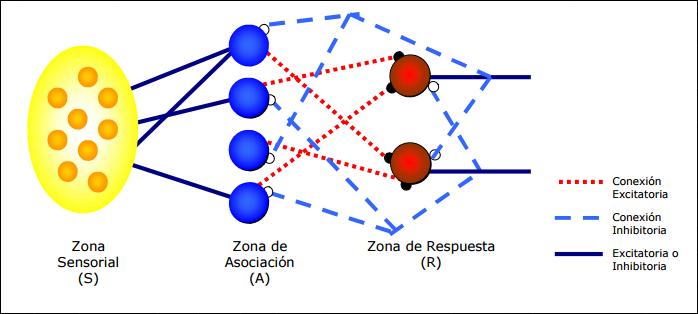
\includegraphics[width=0.95\textwidth]{Fotoperceptron.PNG}
\caption{Fotoperceptron}
\label{Fotoperceptron}
\end{figure}

\begin{itemize}
    \item La luz incide en los puntos sensibles $(S)$ de la estructura de la retina y cada uno de esos puntos responde en forma todo-nada a la luz entrante.
    \item Los impulsos generados por $(S)$ se transmiten a las unidades de asociación $(A)$, donde cada unidad de $(A)$ está conectada a un conjunto aleatorio de puntos de $(S)$. Estas conexiones tienen los valores posibles $+1$, $-1$ y $0$.
    \item Cuando aparece un conjunto de estímulos en la retina $(S)$, una unidad de $(A)$ se activa si la suma de sus entradas sobrepasa algún valor umbral. Si la unidad esta activada, produce una salida que se envía a la siguiente capa de unidades.
    \item De forma similar, las unidades de $(A)$ están conectadas a unidades de respuesta $(R)$ y la conectividad vuelve a ser aleatoria entre ellas.
\end{itemize}

Se pudo demostrar que el Perceptrón era capaz de clasificar patrones correctamente, en lo que Rosenblatt denominaba un entorno diferenciado, en el cual cada clase estaba formada por patrones similares. El Perceptrón también era capaz de responder de manera congruente frente a patrones aleatorios, pero su precisión iba disminuyendo a medida que aumentaba el número de patrones que intentaba aprender.

En 1969 Marvin Minsky y Seymour Papert publicaron su libro: "Perceptrons: An introduction to Computational Geometry", en el que se presentaba un análisis detallado del Perceptrón, en términos de sus capacidades y limitaciones. La mayor desventaja de este tipo de redes es su incapacidad para solucionar problemas que no sean linealmente separables.

Minsky y Papert se apartaban de la aproximación probabilística de Rosenblatt y volvían a las ideas de cálculo de predicados en el análisis del Perceptrón.

La estructura de un Perceptrón sencillo es similar a la siguiente:

\begin{figure}[H]
\centering
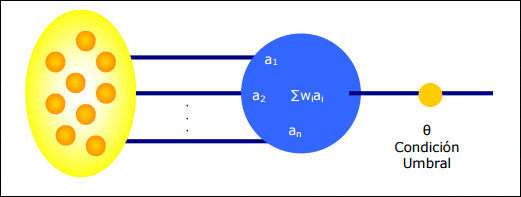
\includegraphics[width=0.7\textwidth]{Perceptron.PNG}
\caption{Estructura Perceptron}
\label{Estructura Perceptron}
\end{figure}

en la cual se observa la adición de una condición umbral en la salida. Si la entrada completa a esta condición es mayor que el valor umbral, la salida de la red es $1$ y en caso contrario es $-1$.

De manera más específica, el Perceptrón se puede definir de la manera siguiente:

\textit{Un \textbf{perceptrón simple} es un dispositivo de computación con umbral $\theta$ y $N$ entradas reales $x_1, ..., x_N$ a través de arcos con pesos $w_1, ..., w_N$ y que tiene salida $1$ cuando $\sum_{i}w_ix_i \geq \theta$ y $-1$ en caso contrario.}

Es decir, supongamos la función  de clasificación $f$ en $\mathbb{R}^n$ tal que:

\[
f(x_1, x_2, ..., x_N) = \left\{ \begin{array}{lcc}
             1 &   si  & w_1x_1 + w_2x_2 + ... + w_Nx_N \geq \theta \\
             \\ -1 &  si  &  w_1x_1 + w_2x_2 + ... + w_Nx_N < \theta 
             \end{array}
   \right.
\]

Dicha función realiza una partición en el espacio $\mathbb{R}^n$ de patrones de entrada: por una parte estarían los patrones con salida $+1$ y por otra parte los patrones con salida $- 1$. Por lo tanto, diremos que la función f clasifica a los patrones de entrada en dos clases.

En este caso, se expresa la función $f$ mediante la función signo, es decir:
\[
f(x_1, x_2, ..., x_N) = sign(x_1, x_2, ..., x_N)
\]

donde la función signo es:
\[
sign(x_1, x_2, ..., x_N) = \left\{ \begin{array}{lcc}
             1 &   si  & x \geq 0 \\
             \\ -1 &  si  &  x < 0 
             \end{array}
   \right.
\]

El algoritmo de aprendizaje del perceptrón consiste en lo siguiente:
\begin{enumerate}
    \item Suponemos que el conjunto de datos es linealmente separable y que se puede encontrar una solución correcta del problema.
    \item El objetivo será buscar el vector $W$ (tal que su hiperplano asociado separe los puntos) que alcanza la solución correcta para todos los puntos.
    \item Suponemos unas salidas esperadas prefijadas $Y_i$ para cada punto a clasificar (con valores $+1$ y $-1$).
    \item \textbf{Paso 1:} Elegir un punto $X_i$ y seleccionar el vector $W_i$ de los pesos en ese momento (al principio dicho vector se podrá inicializar a $0$). Es decir, tenemos las parejas siguientes: ${(X_1, Y_1), ..., (X_N, Y_N)}$ y el algoritmo cogerá un punto que está mal clasificado en ese momento.
    \item \textbf{Paso 2 y sucesivos:} Para el punto $X_i$ seleccionado actualmente, calcular $sign(W^T \times X_i)$.
    \begin{itemize}
        \item Si $sign(W^T \times X_i) \neq Y_i \Rightarrow$ aplicar la regla de actualización $W_{i+1} = W_i + Y_iX_i$.
        \item En caso contrario, volver al paso 2 y continuar el algoritmo con el siguiente punto.
    \end{itemize}
    \item La regla de adaptación de pesos del Perceptrón realiza un movimiento en la dirección correcta para clasificar bien el punto actual $X_i$.
    \item El algoritmo finaliza cuando no haya más puntos mal clasificados.
\end{enumerate}





\subsection{Máquinas y juegos}
En esta sección mencionaremos los años y nombraremos las personalidades que han sido capaces de crear un programa o programas basandose en algoritmos de aprendizaje para que las máquinas sean capaces de aplicar las reglas del juego de una forma lógica y siempre con la intención de ganar.
\subsubsection{Máquinas jugando a las Damas}
En el año 1952 Arthur Samuel que acababa de unirse a un laboratorio de investigación de IBM escribe uno de los primeros programa de aprendizaje automático capaz de jugar a las damas. Se le denomina como un pionero en el campo de juegos de ordenador e inteligencia artificial. El programa de Samuel parece que fue el "primer programa" en el mundo capaz de aprender.

El programa hacía uso de un árbol de juegos basandose en la estrategia minimax principalmente y usando la poda $\alpha\beta$ algoritmos que tratan de anticiparse a lo que hará el contrincante generando un árbol de acciones y podando quedandose con los caminos más probables y eligiendo aquel que obtenga un mayor porcentaje de victoria, pero luego diseñó varios mecanismos que le permitirían mejorar su programa, a estos mecanismos los denomino rote learning o aprendizaje por rutina que es básicamente una técnica que recuerda cada una de las posiciones que ya han sido visitadas basandose en la repeteción y una revaloración del estado de juego.

\subsubsection{Máquinas jugando al Backgammon}
En el año 1992, Gerry Tesauro desarrolla un programa de aprendizaje capaz de jugar al backgammon, basandose en conocimiento obtenido del juego. Esta aplicación del aprendizaje automático fue capaz de jugar casi tan bien como el campeón mundial en el juego. El aprendizaje estaba basado en un algoritmo abreviado TD o temporal difference learning, es un algortimo que trata de realizar predicciones basado en una combinación del método de Monte Carlo y la programación dinámica.

\subsubsection{Máquinas jugando al Ajedrez}
La supercomputadora Deep Blue instalada el año 1996 y desarrollada por IBM era capáz de jugar al ajedrez, lo novedoso de esto es que fue la primera máquina que consiguió vencer una partida al vigente campeón del mundo Gary Kasparov en un encuentro de 6 partidas realizado el mismo año. Sin embargo deep blue no fue capaz de ganar el encuentro debido a que Kasparov gano 4 de los 6 y empató los otros 2. En el año 1997 esta máquina tuvo una considerable mejora pasandose a llamar Deeper Blue que volvio a jugar contra aún vigente campeón del mundo Kasparov de nuevo en un encuentro a 6 partidas donde esta vez ganó Deeper blue con 3 victorias 2 derrotas y 1 empate.

\subsubsection{Máquinas jugando al go}
En el año 2015 Google DeepMind de Londres desarrolla un programa de ordenador llamado AlphaGo capaz de jugar al juego Go. Que resulta ser el primer programa que juega a ese juego en derrotar una persona profesional en un tablero de 19x19. El juego Go es considerado mucho más dificil de tratar computacionalmente que otros juegos como el ajedrez debido a que se tiene una gran cantidad de opciones y por tanto un gran árbol de decisión generado. Esto hace que los típicos algoritmos como la poda $\alpha\beta$ y otros métodos de búsqueda sean difíciles de usar, la capacidad de aprendizaje del programa se basa en una red neuronal que usa deep learning. El deep learning es una rama del machine learning que toma un conjunto de algoritmos que intentan obtener un modelo de abstracciones sobre los datos.

\subsection{Nearest Neighbor}
\subsection{Stanford cart y otros experimentos}
\subsection{Neocognitron}
\subsection{Backpropagation}
\subsection{Algoritmos de aprendizaje}
\subsection{Final con el estado actual del machine learning}
Esto va a ser una recopilación de los finales que encontreis para cada área.
\begin{thebibliography}{9}

 \bibitem{Timeline}
 \url{https://en.wikipedia.org/wiki/Timeline_of_machine_learning}

\bibitem{articulointro}
 	\textbf{Introducción},
 \url{http://cleverdata.io/que-es-machine-learning-big-data/}
 
 \bibitem{conceptosbasicos}
 	\textbf{Introducción},
 \url{ftp://decsai.ugr.es/pub/usuarios/castro/Actividades/Redes-Neuronales/Apuntes/Apuntes%20Javier%20Rodriguez%20Blazquez/Conceptos%20basicos.pdf}

\bibitem{standford1}
	\textbf{Neural Networks},
  \url{http://cs.stanford.edu/people/eroberts/courses/soco/projects/neural-networks/History/history2.html}
 
 \bibitem{standford2}
 	\textbf{Neural Networks},
 \url{http://cs.stanford.edu/people/eroberts/courses/soco/projects/neural-networks/History/history1.html}
 
 \bibitem{wikiNN1}
 	\textbf{Neural Networks},
 \url{https://en.wikipedia.org/wiki/Artificial_neural_network}
 
 \bibitem{marvinminsky}
 	\textbf{Neural Networks},
 \url{https://en.wikipedia.org/wiki/Marvin_Minsky}
 
 \bibitem{historiademachinelearning}
 	\textbf{Perceptrón},
 \url{http://sge.wonderville.ca/machinelearning/history/history.html}
 
 \bibitem{perceptron1}
 	\textbf{Perceptrón},
 \url{http://www.lcc.uma.es/~jmortiz/archivos/Tema4.pdf}
 
 \bibitem{perceptron2}
 	\textbf{Perceptrón},
 \url{ftp://decsai.ugr.es/pub/usuarios/castro/Actividades/Redes-Neuronales/Apuntes/Apuntes%20Javier%20Rodriguez%20Blazquez/Redes%20de%20una%20capa.pdf}
 
 
 

\end{thebibliography}
\end{document}